\documentclass [12pt] {article}
\makeatletter
\setlength{\@fptop}{0pt}
\makeatother
\usepackage{graphicx}
\usepackage{color}
\usepackage{listings}
\lstset{ %
language=C++,                % choose the language of the code
basicstyle=\footnotesize,       % the size of the fonts that are used for the code
numbers=left,                   % where to put the line-numbers
numberstyle=\footnotesize,      % the size of the fonts that are used for the line-numbers
stepnumber=1,                   % the step between two line-numbers. If it is 1 each line will be numbered
numbersep=5pt,                  % how far the line-numbers are from the code
backgroundcolor=\color{white},  % choose the background color. You must add \usepackage{color}
showspaces=false,               % show spaces adding particular underscores
showstringspaces=false,         % underline spaces within strings
showtabs=false,                 % show tabs within strings adding particular underscores
frame=single,           % adds a frame around the code
tabsize=2,          % sets default tabsize to 2 spaces
captionpos=b,           % sets the caption-position to bottom
breaklines=true,        % sets automatic line breaking
breakatwhitespace=false,    % sets if automatic breaks should only happen at whitespace
escapeinside={\%*}{*)}          % if you want to add a comment within your code
}

\title{\vspace{-2cm}Assignment \#: Silver Springs Model}
\author{Timmy Nguyen}
\begin{document}
\maketitle
\section{A Brief Introduction}
In this model, 
\section{Results}

\subsubsection{Compartment Model}
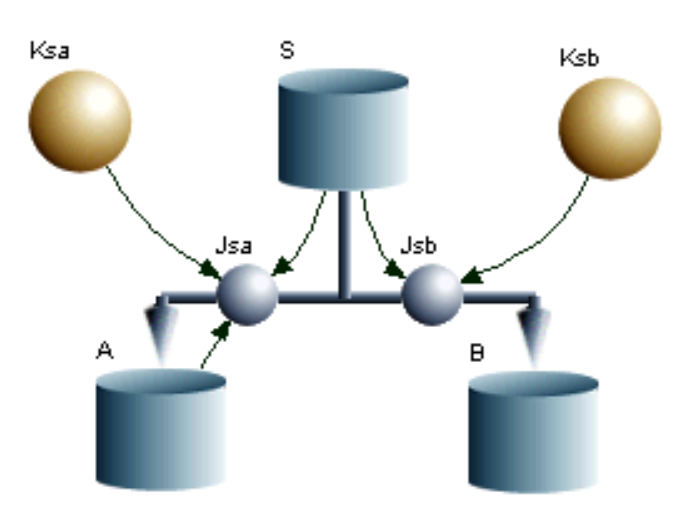
\includegraphics[scale=1.6]{compartment_model.PNG} \\
% 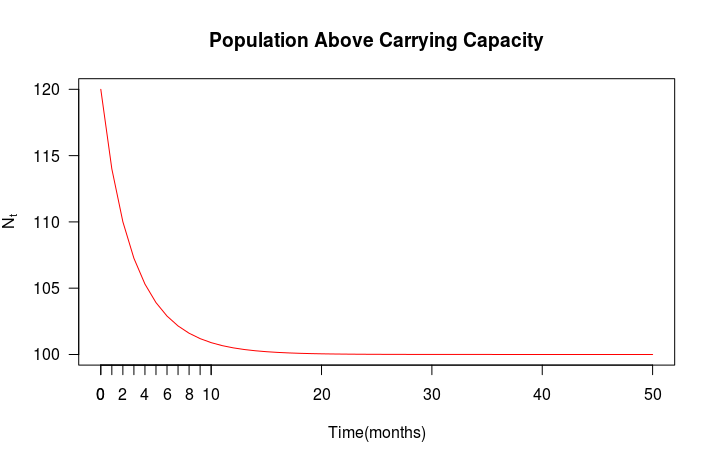
\includegraphics[scale=0.6]{graph2.png}
\newpage


\subsubsection{Flow vs Time}
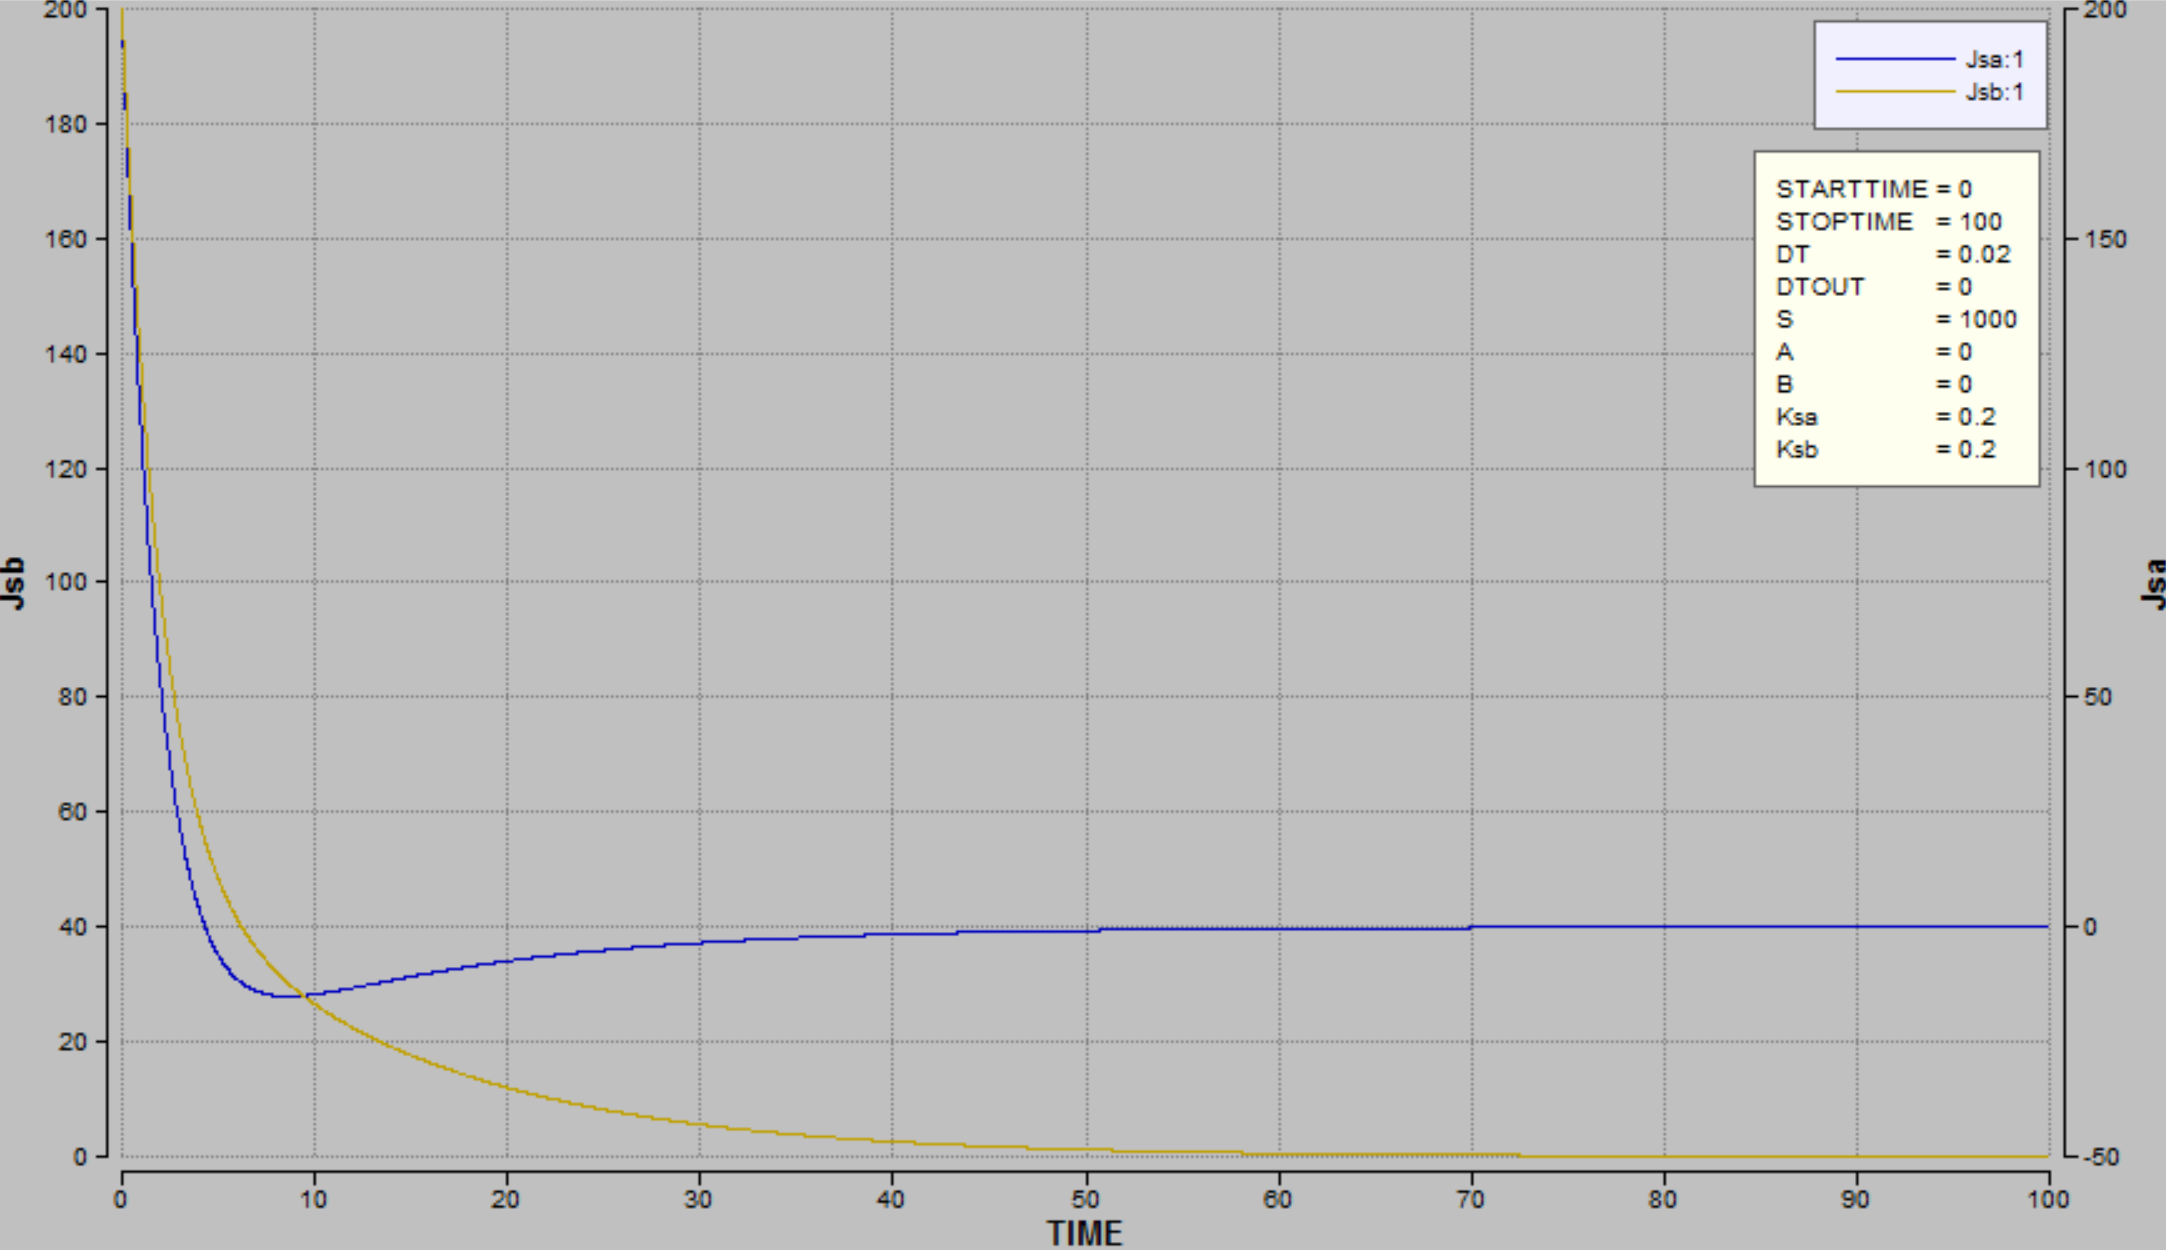
\includegraphics[scale=0.7]{flow_vs_time.PNG} \\

\subsection{Reservoir level Over Time}
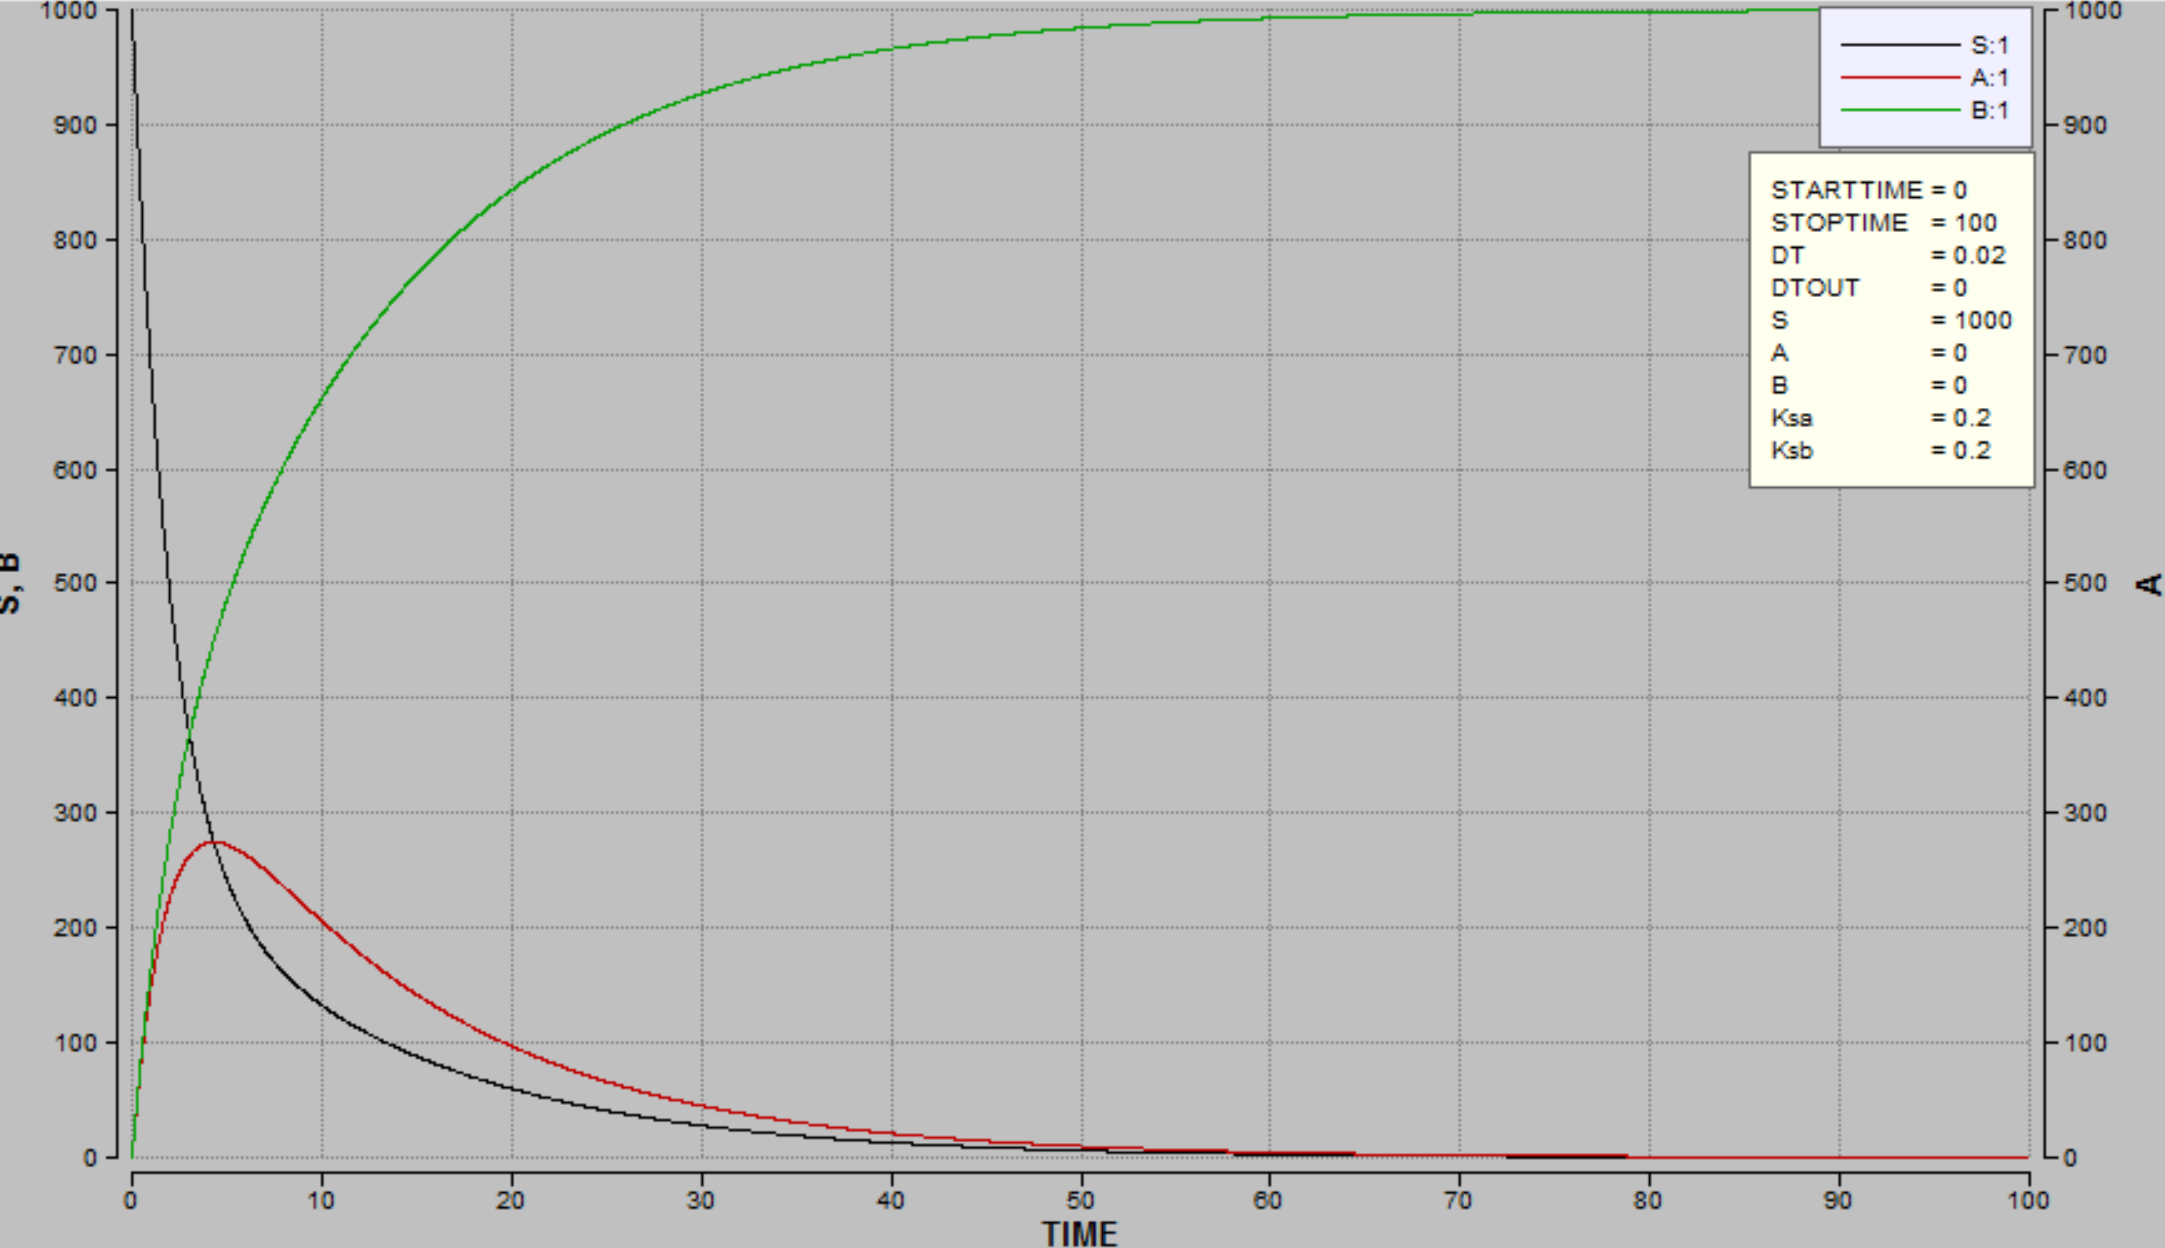
\includegraphics[scale=0.7]{SAB_vs_Time.PNG}

\subsection{Ksb $>$  Ksa}
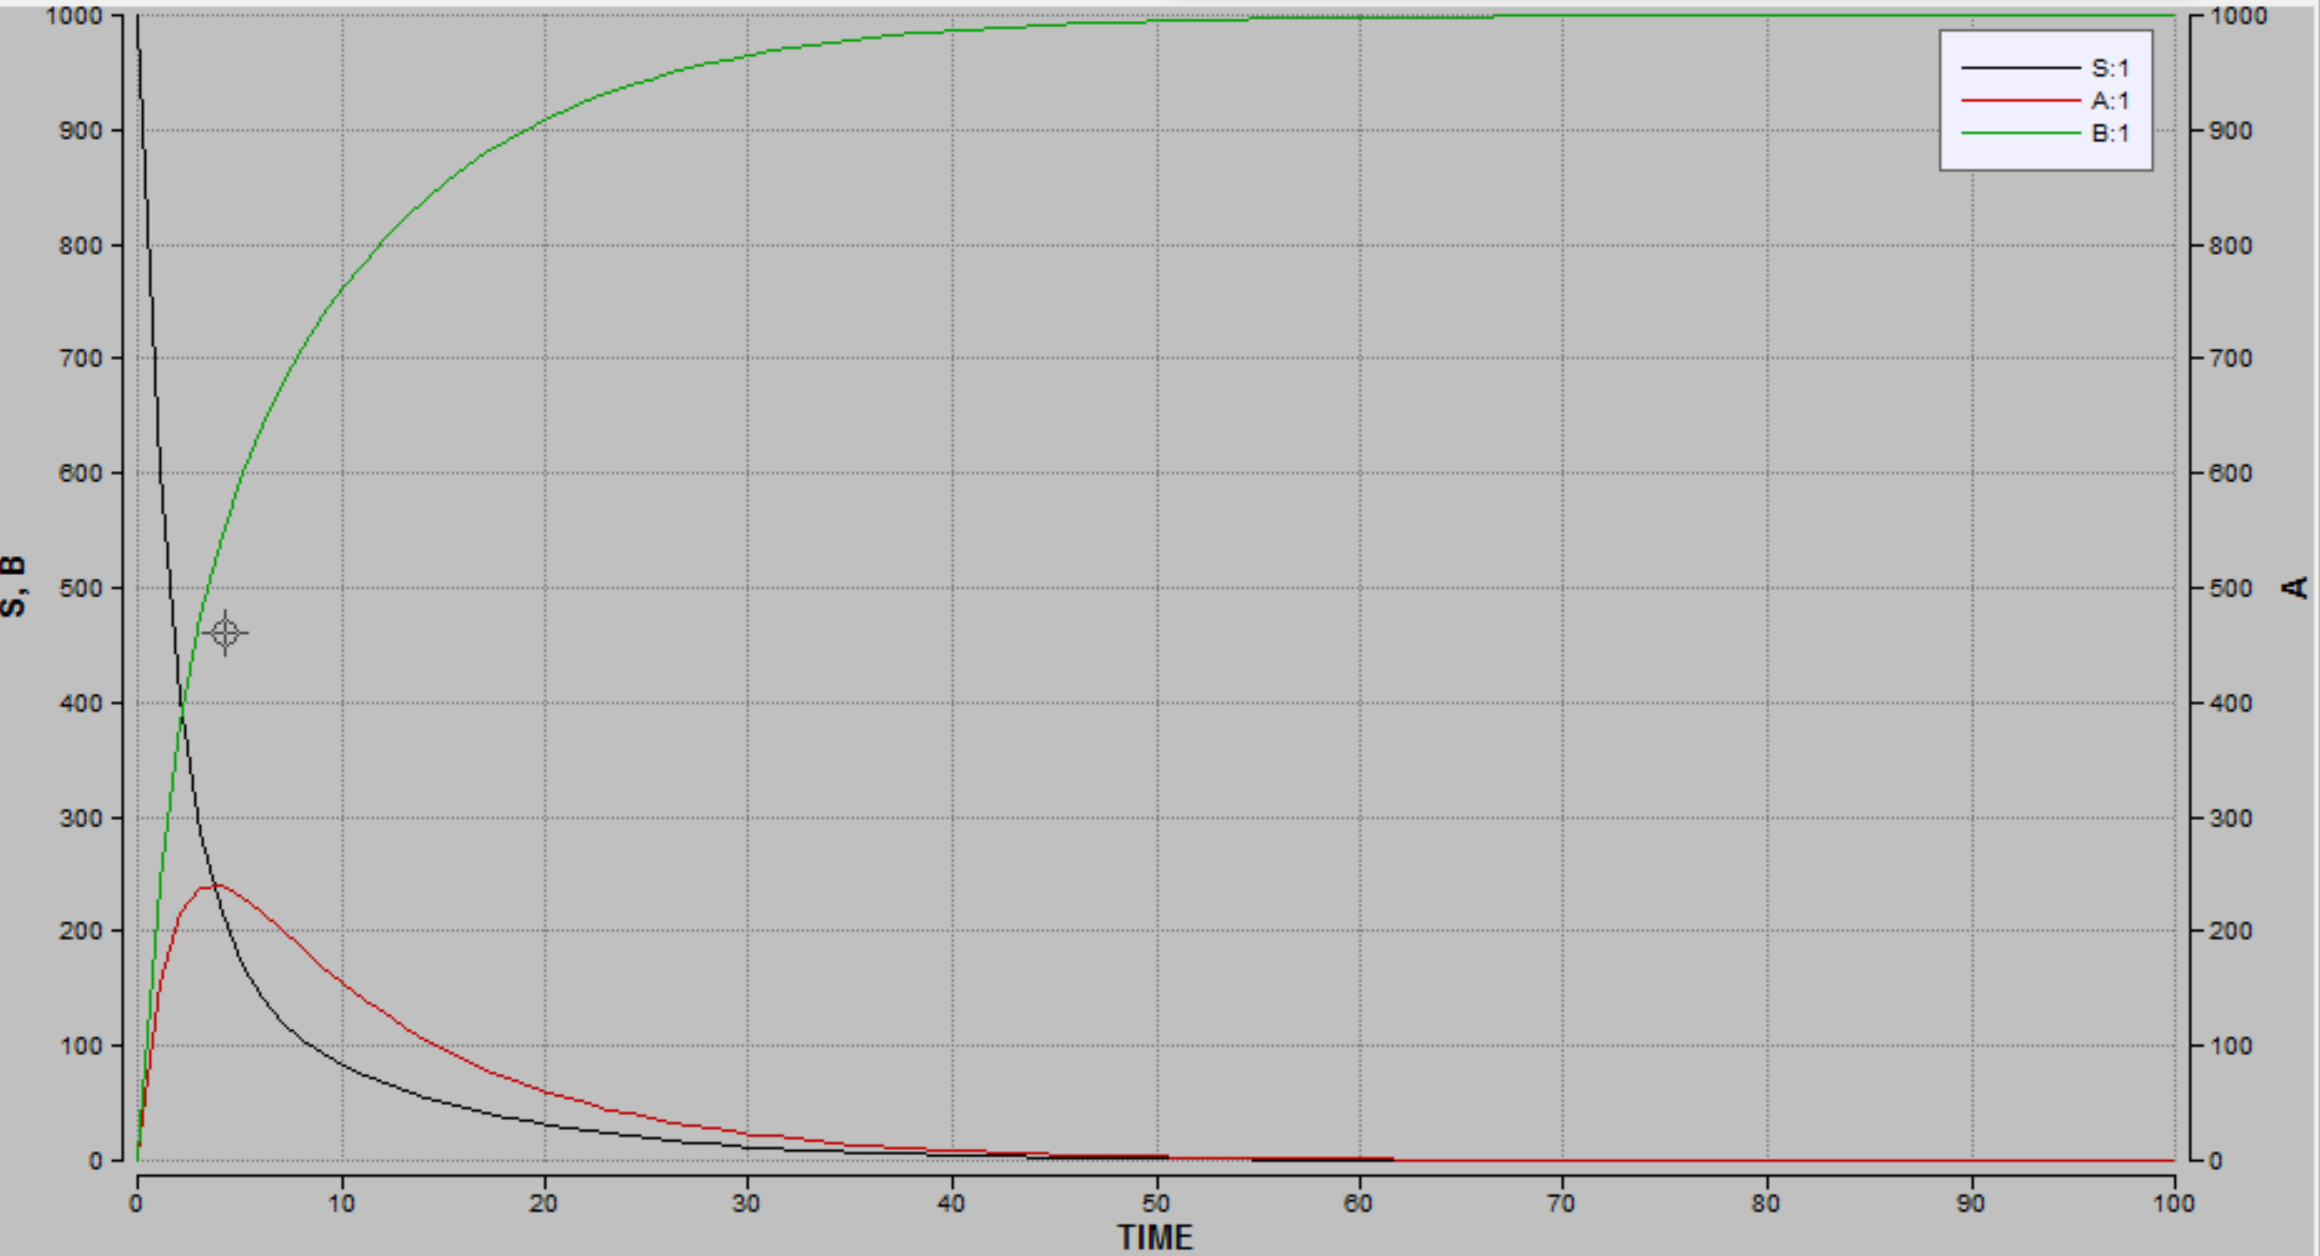
\includegraphics[scale=0.7]{ksb_greater_ksa.PNG}

\subsection{Ksb $<$ Ksa}
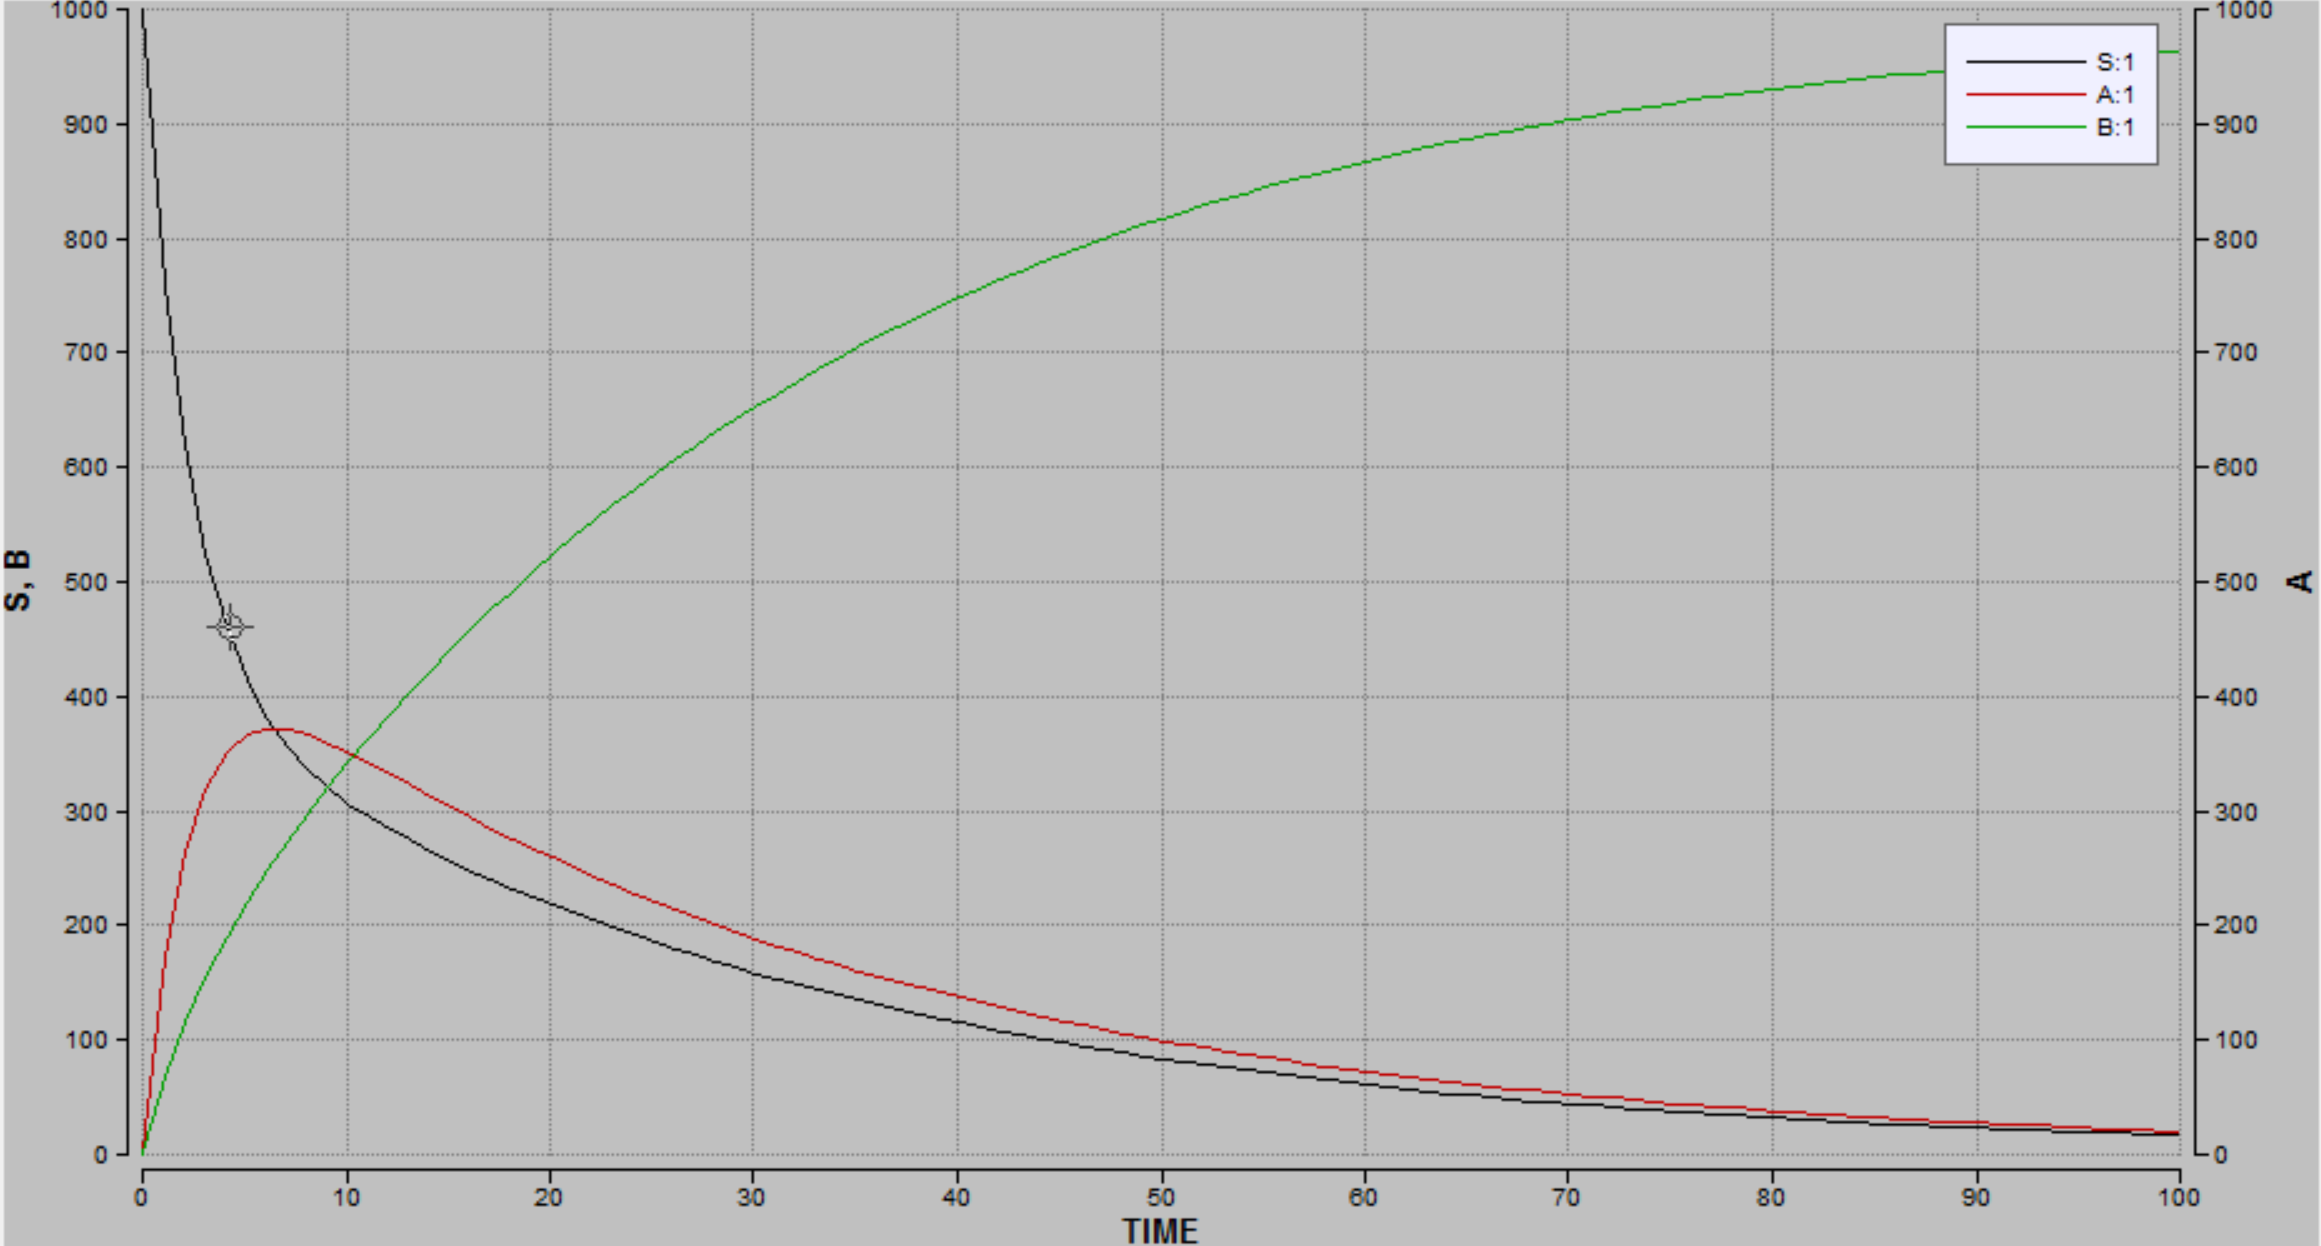
\includegraphics[scale=0.7]{ksb_less_ksa.PNG}


\section{Conclusion}
From my observations, when the graph of \textit{S} intersects with a graph from either \textit{A} or \textit{B}, it presents an equilibrium of the two compartment volume. When the $K_{sb}$ value is greater than the $K_{sa}$, compartment B fills up at a faster pace.  When the $K_{sb}$ value is less than the $K_{sa}$, compartment \textit{A} will have a higher volume than \textit{B} up to when the graph of A intersects with the graph of B. In conclusion, when S decreases both graph of A and B increases; however, the graph of A will began to decrease when it intersects with S.
\newpage

\section{Appendix}
% \subsubsection{C/C++ Code for Exponential Growth Model}
% \lstinputlisting[language=c]{Predator_Prey_model.cpp}
% \subsubsection{R Code for Generating Predator and Prey Population Size Over Time}
% \lstinputlisting[language=R]{Predator_Prey_Model.R}

% \subsectio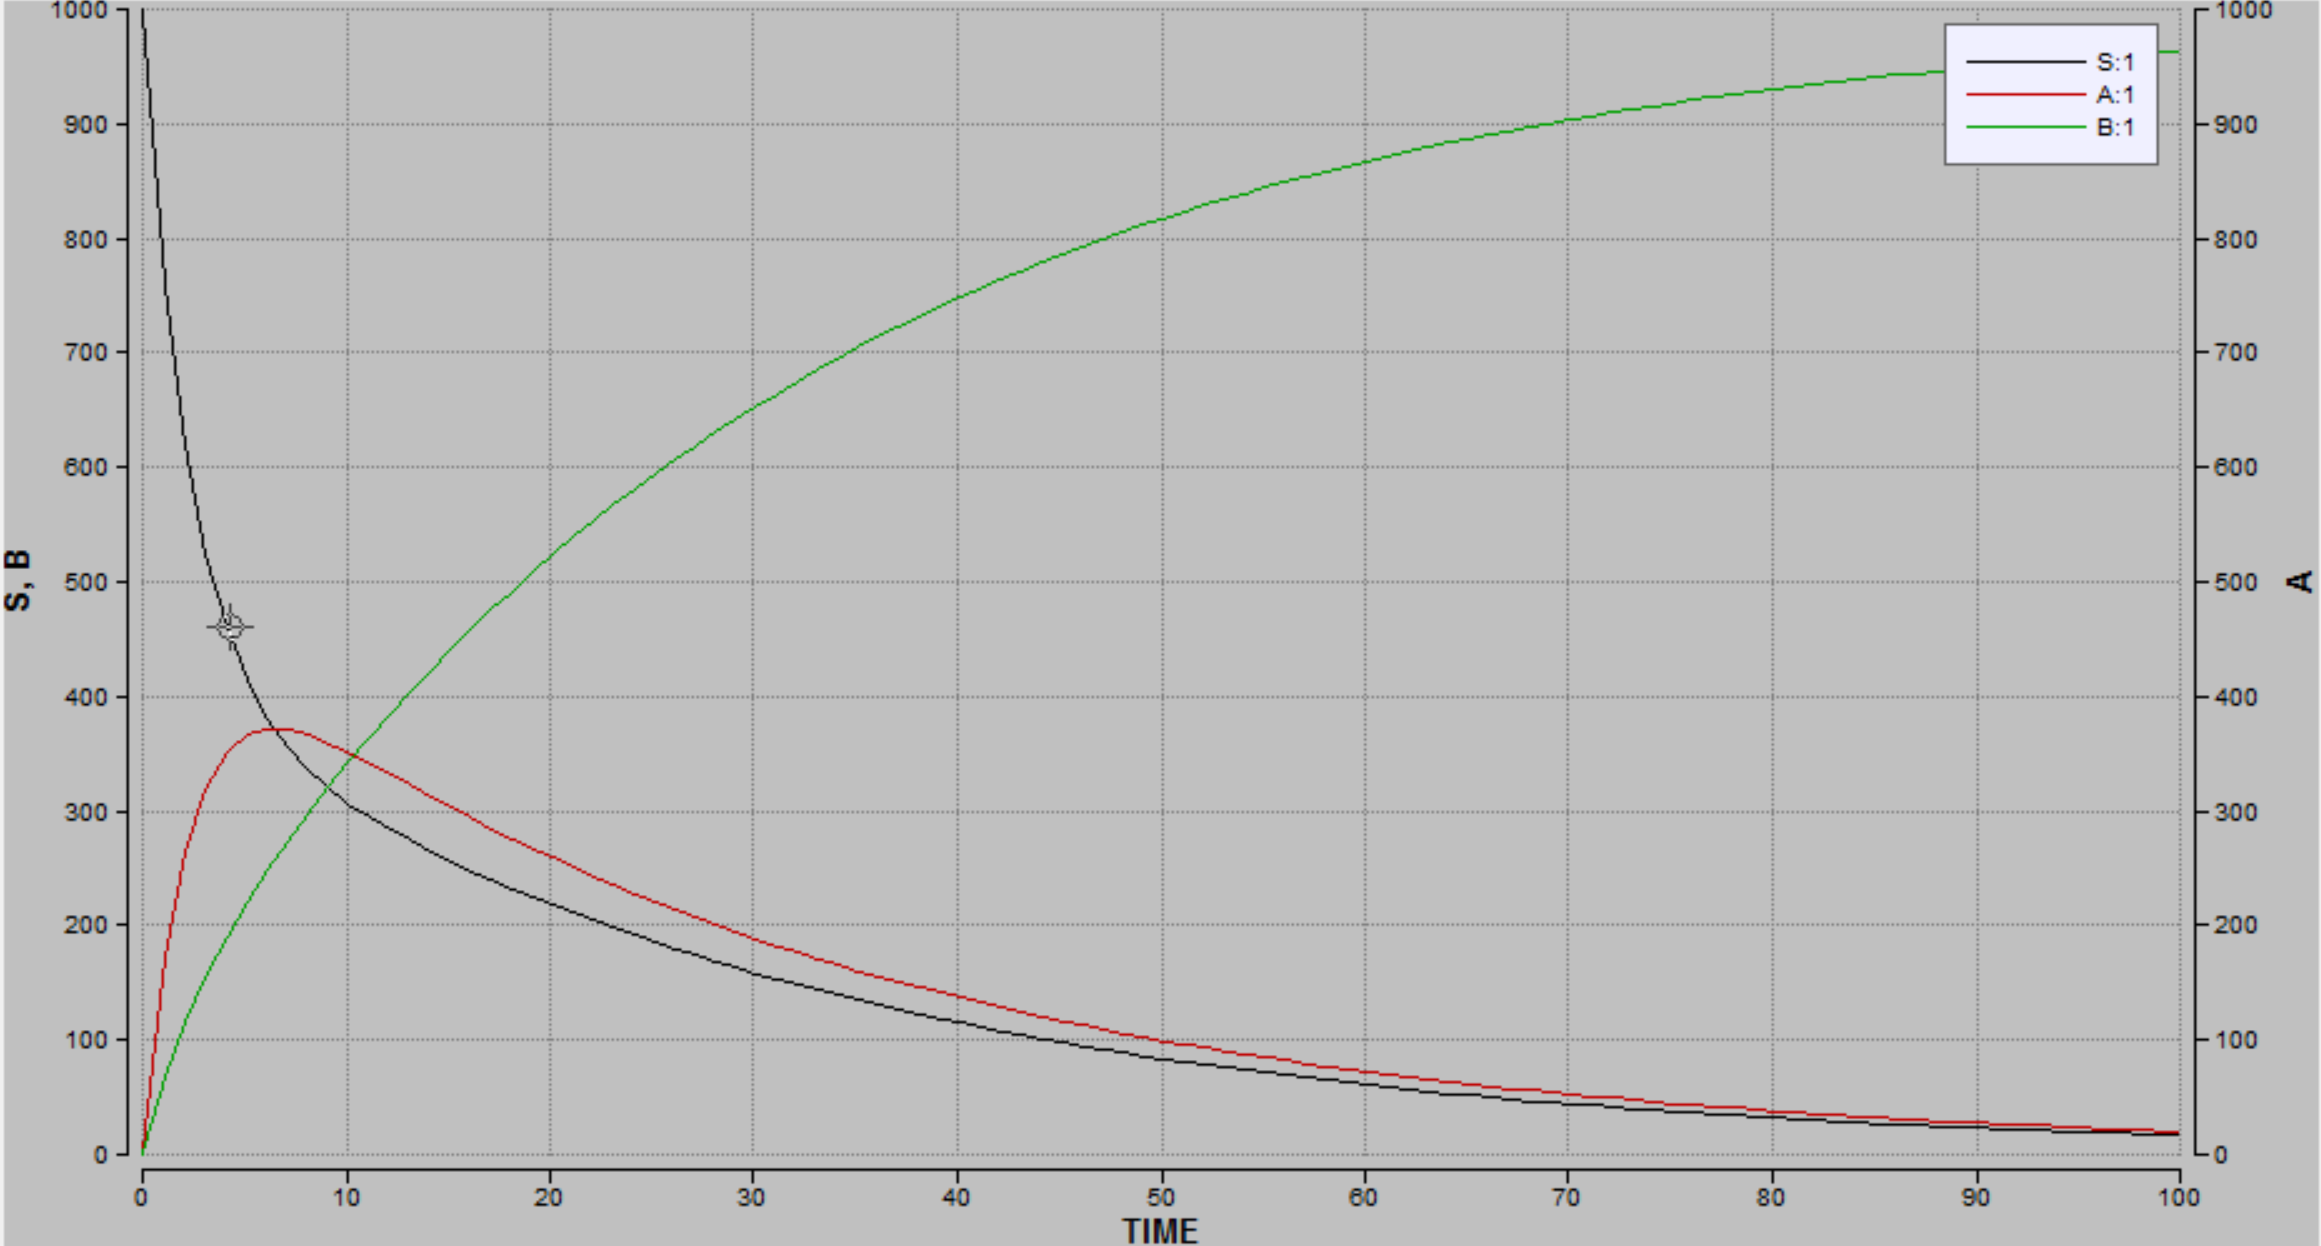
\includegraphics[scale=0.7]{ksb_less_ksa.PNG}n{R code for Generating Predator vs Prey Population Size }
% \lstinputlisting[language=R]{Predator_VS_Prey_Graph.R}
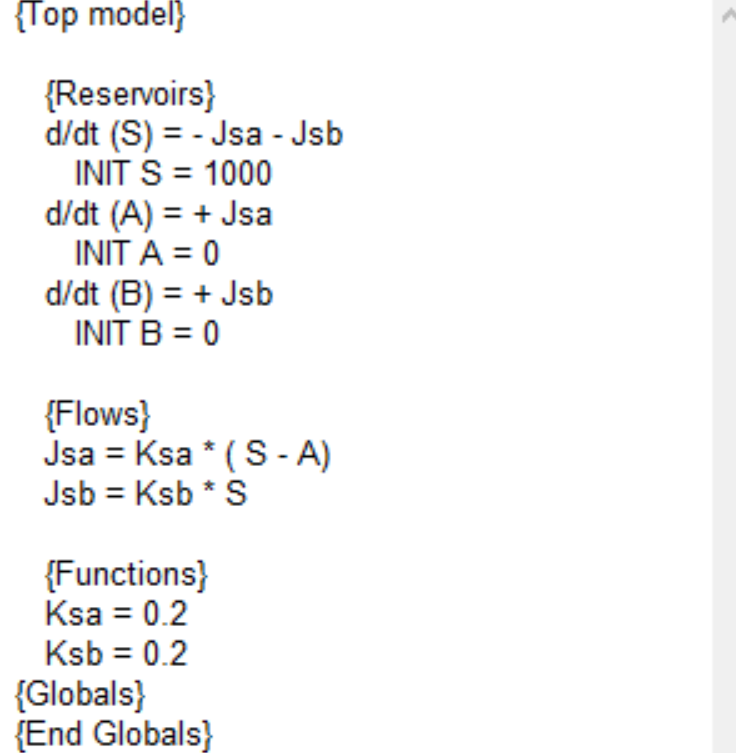
\includegraphics[scale=2.0]{compartment_equations.PNG}

\end{document}

